\section{Coherencia del sistema de memoria}

\subsection{Sistema de memoria en multiprocesadores}

En las arquitecturas multiprocesador, el sistema de memoria está compuesto por las cachés de todos los nodos que la conforman, la memoria principal, los controladores, los buffers (de escritura/almacenamiento o que las combinan) y el medio de comunicación de todos estos componentes, al que llamamos \textbf{red de interconexión}.
Este sistema de memoria es quien realiza la comunicación de datos entre los procesadores, de forma que la lectura de una dirección devuelve siempre lo último que se ha escrito en ella (como ocurre normalmente).

\subsection{Concepto de coherencia en el sistema de memoria}

\subsubsection{Situaciones de incoherencia en el sistema de memoria}

\begin{center}
\begin{tabular}{p{6cm} p{6cm} p{6cm}}
\textbf{Clases de estructuras de datos} & \textbf{Efentos que ponen de manifiesto faltas de coherencia} & \textbf{Tipos de falta de coherencia} \\
\toprule
Datos modificables & E/S & Caché-MP \\
\multirow{2}{*}{Datos modificables compartidos} & Lectura de caché no actualizada & Caché-Caché \\
                                                & Fallo de caché & Caché-MP \\
Datos modificables privados & Emicra hebra/proceso $\rightarrow$ Fallo de caché & Caché-MP \\
\end{tabular}
\end{center}

\subsubsection{Métodos de actualización de memoria principal implementados en cachés}

Si la actualización se hace mediante \textbf{escritura inmediata} (\textit{write-through}), cada vez que un procesador escribe en su caché, escribe también en memoria principal.
Sin embargo, por los principios de localidad temporal y espacial resulta más rantable escribir todo el bloque una vez realizadas varias escrituras.
Por ello existe la \textbf{posescritura} (\textit{write-back}), mediante la cual se actualiza la memoria principal escribiendo todo el bloque cuando se desaloja la caché.

\subsubsection{Alternativas para propagar una escritura en protocolos de coherencia de caché}

Mediante una \textbf{escritura con actualización} (\textit{write-update}), cada vez que un procesador escribe en una dirección de su caché se escribe en las copias de esa dirección en otras cachés.
Sin embargo, esto da lugar a una gran cantidad de tráfico de datos.
Para reducirlo, sobre todo si los datos están compartidos por pocos procesadores, podemos usar una \textbf{escritura con invalidación} (\textit{write-invalidate}), que invalida las copias del bloque de la dirección en otras cachés antes de modificar la suya, de forma que se debe acceder al dato en la caché del procesador que envió la invalidación.

\subsubsection{Situación de incoherencia aún con propagación de escrituras}

Supongamos que tenemos cuatro procesadores $P_{0-3}$.
El procesador $P_0$ escribe $1$ en la variable $x$ y, justo después, $P_1$ escribe $2$ en esta misma variable.
Ambos procesadores propagan la escritura al resto de cachés, de forma que $P_0$ propaga a $P_1$, $P_2$ y $P_1$ propaga a $P_0$, $P_2$ y $P_3$.

\begin{figure}[h]
\begin{center}
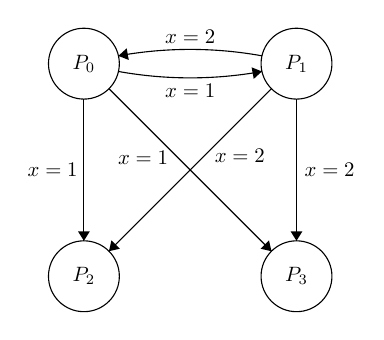
\begin{tikzpicture}[scale=0.15, every node/.style={scale=0.75}]
\tikzstyle{every node}+=[inner sep=0pt]
\draw [black] (3.8,-3.6) circle (3);
\draw (3.8,-3.6) node {$P_0$};
\draw [black] (21.8,-3.6) circle (3);
\draw (21.8,-3.6) node {$P_1$};
\draw [black] (21.8,-21.6) circle (3);
\draw (21.8,-21.6) node {$P_3$};
\draw [black] (3.8,-21.6) circle (3);
\draw (3.8,-21.6) node {$P_2$};
\draw [black] (6.725,-2.937) arc (100.24617:79.75383:34.153);
\fill [black] (6.72,-2.94) -- (7.6,-3.29) -- (7.42,-2.3);
\draw (12.8,-1.89) node [above] {$x=2$};
\draw [black] (19.68,-5.72) -- (5.92,-19.48);
\fill [black] (5.92,-19.48) -- (6.84,-19.27) -- (6.13,-18.56);
\draw (17,-12) node [above] {$x=2$};
\draw [black] (21.8,-6.6) -- (21.8,-18.6);
\fill [black] (21.8,-18.6) -- (22.3,-17.8) -- (21.3,-17.8);
\draw (26.75,-12.6) node [left] {$x=2$};
\draw [black] (18.875,-4.261) arc (-79.78374:-100.21626:34.249);
\fill [black] (18.87,-4.26) -- (18,-3.91) -- (18.18,-4.89);
\draw (12.8,-5.3) node [below] {$x=1$};
\draw [black] (3.8,-6.6) -- (3.8,-18.6);
\fill [black] (3.8,-18.6) -- (4.3,-17.8) -- (3.3,-17.8);
\draw (3.3,-12.6) node [left] {$x=1$};
\draw [black] (5.92,-5.72) -- (19.68,-19.48);
\fill [black] (19.68,-19.48) -- (19.47,-18.56) -- (18.76,-19.27);
\draw (8.8,-11) node [below] {$x=1$};
\end{tikzpicture}

\end{center}
\caption{Modelo propuesto de propagación de escrituras}
\end{figure}

Debido al tiempo de propagación, el valor de $x$ llega en distinto orden a los procesadores (que suponemos todos en la misma placa).
Por ejemplo, $P_0$ y $P_2$ registran que $x=2$ mientra sque $P_1$ y $P_3$, que $x=1$.

\subsubsection{Requisitos del sistema de memoria para evitar problemas de incoherencia}

El sistema de \textbf{propagar las escrituras en una dirección}, es decir, esta escritura debe hacerse visible en un tiempo finito a otros procesadores.


\subsection{Protocolos de mantenimiento y coherencia}

\subsection{Protocolo MSI de espionaje}

\subsection{Protocolo MESI de espionaje}

\subsection{Protocolo MSI basado en directorios con o sin difusión}
